% !TeX TS-program = pdflatex
% !TeX encoding = UTF-8
% !TeX spellcheck = en_GB
% !TeX root = optarticle.tex
\documentclass[10pt,a4paper,fleqn]{article}
% -------------------------------- %
%\usepackage{lmodern}
\usepackage{cfr-lm}
\usepackage[T1]{fontenc}
\usepackage{textcomp}
\usepackage[utf8]{inputenc}
\usepackage[UKenglish]{babel}
%\hyphenation{}
\usepackage{microtype}
\usepackage{indentfirst}
\usepackage[heightrounded]{geometry}
\usepackage{lipsum}
% -------------------------------- %
% Math
% -------------------------------- %
\usepackage{amsmath}
\usepackage{amssymb}
\usepackage{mathtools}
\usepackage{amsthm}
% -------------------------------- %
\newcommand{\numberset}{\mathbb}
%\newcommand{\N}{\numberset{N}}
\newcommand{\R}{\numberset{R}}
% -------------------------------- %
\renewcommand{\epsilon}{\varepsilon}
%\renewcommand{\theta}{\vartheta}
%\renewcommand{\rho}{\varrho}
%\renewcommand{\phi}{\varphi}
% -------------------------------- %
\DeclarePairedDelimiter{\abs}{\lvert}{\rvert}
\DeclarePairedDelimiter{\norma}{\lVert}{\rVert}
\DeclarePairedDelimiter{\set}{\{}{\}}
% -------------------------------- %
%\DeclareMathOperator{\sgn}{sgn}
%\DeclareMathOperator{\Realpart}{Re}
%\renewcommand{\Re}{\Realpart}
%\DeclareMathOperator*{\argmax}{arg\,max}
%\DeclareMathOperator*{\argmin}{arg\,min}
%\DeclareMathOperator{\Loss}{\mathit{L}}
\DeclareMathOperator{\loss}{\ell}
%\DeclareMathOperator{\regul}{\Omega}
\DeclareMathOperator*{\func}{\mathit{f}}
%\DeclareMathOperator*{\gradF}{\nabla\mathit{f}} % check if it works fine
%\DeclareMathOperator*{\hessF}{\nabla^2\mathit{f}}
%\DeclareMathOperator*{\Var}{Var}
%\DeclareMathOperator*{\bigO}{\mathcal{O}}
% -------------------------------- %
% Definitions
\theoremstyle{definition}
\newtheorem{defs}{Definition}
%\newtheorem{propts}{Property}
% Theorems
\theoremstyle{plain}
\newtheorem{thm}{Theorem}
\newtheorem{cor}[thm]{Corollary}
\newtheorem{prop}{Proposition}
%\newtheorem{lem}[thm]{Lemma}
\renewcommand{\qedsymbol}{$\blacksquare$}
% Remarks
\theoremstyle{remark}
\newtheorem{rmk}{Remark}
% -------------------------------- %
% Numbers
% -------------------------------- %
\usepackage{siunitx}
\sisetup{%
	output-decimal-marker={.},group-separator={\,},%
%	round-mode=places,round-precision=6,%
	table-parse-only,table-number-alignment=center%
}
% -------------------------------- %
% Tikz and colors
% -------------------------------- %
%\usepackage{xcolor}
%\usepackage{pgf}
\usepackage{pgfplots} % + tikz
%\pgfplotsset{/pgf/number format/use comma,compat=newest}
\pgfplotsset{compat=newest}
\usetikzlibrary{calc}
%%\usepackage{tikz} % + graphicx,keyval,xcolor
%%\definecolor{Maroon}{cmyk}{0,0.87,0.68,0.32}
\definecolor{RoyalBlue}{cmyk}{1,0.50,0,0}
%%\definecolor{halfgray}{gray}{0.55}
\definecolor{webgreen}{rgb}{0,0.5,0}
\definecolor{webbrown}{rgb}{0.6,0,0}
\definecolor{lightergray}{gray}{0.99}
% -------------------------------- %
% Floating objects
% -------------------------------- %
%\usepackage{import}
\usepackage{booktabs}
\usepackage{tabularx}
%\usepackage{multirow}
\graphicspath{{./Figures/},{../py/plots/}}
\usepackage{subfig}
%\usepackage{wrapfig}
\usepackage{caption}
\captionsetup{format=hang,labelsep=colon,font={small,rm},labelfont={sf,bf}}
\captionsetup[table]{skip=0.2\medskipamount,position=top}
\captionsetup[figure]{position=bottom}
\usepackage{flafter}
\usepackage[english,nospace]{varioref}
%\usepackage{enumitem}
% -------------------------------- %
% Code
% -------------------------------- %
\usepackage{listings}
% -------------------------------- %
%% R programming language
\definecolor{Rkwd}{rgb}{0.737,0.353,0.396}
\definecolor{Rparam}{rgb}{0.333,0.667,0.333}
\definecolor{Rnum}{rgb}{0.686,0.059,0.569}
\definecolor{Rstr}{rgb}{0.192,0.494,0.8}
\definecolor{Rcomm}{rgb}{0.678,0.584,0.686}
\lstdefinestyle{Rlang}{language=R,%
	keywordstyle=\color{Rkwd},basicstyle=\small\ttfamily,%
	commentstyle=\color{Rcomm}\ttfamily\em,%
	stringstyle=\color{Rstr}\rmfamily,%
	numbers=left,numberstyle=\tiny,stepnumber=1,numbersep=5pt,%
	showstringspaces=false,breaklines=true,frameround=ftff,%
	frame=lines,backgroundcolor=\color{lightergray},firstnumber=last%
	%	deletekeywords={}
}
% -------------------------------- %
% Python programming language
\lstdefinestyle{Pylang}{language=Python,%
	basicstyle=\small\ttfamily,%
	keywordstyle=,commentstyle=,stringstyle=,%
	numbers=left,numberstyle=\tiny,stepnumber=1,numbersep=5pt,%
	showstringspaces=false,breaklines=true,%
	frameround=ftff,frame=lines,%
	backgroundcolor=\color{lightergray},%
%	firstnumber=last,%
}
% -------------------------------- %
% Code output
\lstdefinestyle{output}{%
	basicstyle=\scriptsize\ttfamily,%
	showstringspaces=false,breaklines=true,frameround=ftff,%
	frame=lines,backgroundcolor=\color{lightergray},%
	%	deletekeywords={}
}
% -------------------------------- %
% Pseudo-code
\lstdefinestyle{simple}{%
	basicstyle=\small\ttfamily,%
	keywordstyle=\color{black}\bfseries,%
	commentstyle=\color{darkgray},%
	stringstyle=\color{black},%
	numbers=left,numberstyle=\tiny,stepnumber=1,numbersep=5pt,%
	showstringspaces=false,breaklines=true,frameround=ftff,%
	frame=lines,backgroundcolor=\color{lightergray},%
	escapeinside={£!}{!£},%
	morekeywords={while,end,poni,dati,return,for},%
	%	comment={//},%
}
% -------------------------------- %

\usepackage[ruled,linesnumbered]{algorithm2e}
\SetNlSty{texttt}{}{}
\SetKw{Or}{or}
\SetKw{And}{and}
\SetKw{Not}{not}
% -------------------------------- %
% Miscellaneous
% -------------------------------- %
\interfootnotelinepenalty=10000
\dimen\footins=2.5cm
\renewcommand{\thefootnote}{\fnsymbol{footnote}}
% -------------------------------- %
% My stuff
% -------------------------------- %
\newcommand{\myTitle}{Stochastic Gradient Descent with Momentum and Line Searches}
\newcommand{\mySubject}{Project work in Optimization Techniques for Machine Learning}
\newcommand{\myName}{David Nardi}
\newcommand{\myNameShort}{D. Nardi}
\newcommand{\mySummary}{MSc student in Artificial Intelligence\\ Univeristy of Florence}
\newcommand{\omissis}{[\textellipsis\unkern]}
\newcommand{\inToc}[1]%
	{\addcontentsline{toc}{section}{\texorpdfstring{\protect\numberline{}#1}{#1}}}
% -------------------------------- %
\title{\myTitle}
\author{\myName\\ \mySummary}
%\date{}
% -------------------------------- %
% Page styles
% -------------------------------- %
\usepackage{titleps}
\newpagestyle{main}{% oneside mainmatter
	\sethead[][][]%
	{\slshape\myNameShort}{}{\slshape\myTitle}%
	\setfoot[][][]%
	{}{\thepage}{}}
% -------------------------------- %
% Bibliography
% -------------------------------- %
\usepackage[autostyle,italian=guillemets,babel]{csquotes}
\usepackage[backend=biber,useprefix,style=ieee,backref,hyperref,defernumbers=true]{biblatex}
%\usepackage[backend=biber,useprefix,style=authoryear-comp,hyperref,defernumbers=true]{biblatex}
\addbibresource{optarticle-bib.bib}
% -------------------------------- %
\usepackage[hyperfootnotes=false]{hyperref}
\hypersetup{%
	colorlinks,urlcolor=webbrown,linkcolor=RoyalBlue,citecolor=webgreen,%
	linktocpage,pdfstartpage=1,bookmarksnumbered,bookmarksopen,bookmarksopenlevel=2,%
	pdftitle={\myTitle},pdfauthor={\myName},pdfsubject={\mySubject}%
}
% -------------------------------- %
%\usepackage{showframe}
\begin{document}
\frenchspacing
% ************************************************************************************* %
% FRONTMATTER
% ************************************************************************************* %
\cleardoublepage
\pdfbookmark[1]{Title page}{fronte}
\maketitle

\begin{abstract}
In recent years, tailored line search approaches have proposed to define the step-size, or learning rate, in SGD-type algorithms for finite-sum problems. In particular, a stochastic extension of standard Armijo line search has been proposed in~\textcite{vaswani_painless_2019}. The development of this kind of techniques is relevant, because it shall allow to enforce a stronger converging behaviour (due to the Armijo condition), similar to that of standard GD, within SGD methods that are commonly employed with large scale training problems.

However, the stochastic line search is not immediately employable when the momentum term is part of the update equation, as the search direction might not be a descent direction (which is a necessary condition for the Armijo condition). This problem is addressed in~\textcite{fan_msl_2023}, where a strategy is proposed to guarantee the descent property with momentum.
\end{abstract}

\setcounter{tocdepth}{2}
\tableofcontents\cleardoublepage
\pagestyle{main}
% ************************************************************************************* %
% MAINMATTER %
% ************************************************************************************* %
% !TeX spellcheck = en_GB
% ***************************************************** %
\section{Introduction}\label{sc:intro}
% ***************************************************** %

% problem identification
% solutions

This report summarizes the analysis performed in order to investigate the behaviour of the algorithms retrieved from the scientific literature. The optimization problem that we aim to solve is that of the Logistic Regression with $\ell_2\text{-regularization}$ term added.

Follows a list of the suggested algorithms from the literature, since those methods share many computations, we decided to implement just two algorithms
\begin{itemize}
\item Mini-batch Gradient Descent with fixed step-size and momentum, and decreasing step-size, algorithm~\vref{alg:SGD-F-D-M};
\item Mini-batch Gradient Descent with Armijo line search and momentum restart or correction, algorithm~\vref{alg:SGD-SLS-M};
\end{itemize}

After that, the efficiency of the algorithms is tested on different datasets.

In this section the Machine Learning (ML) problem and the relative optimization problem are shown shown, proving the existence and uniqueness of the optimal solution.

% ---------------------------------------------------- %
\subsection{Classification task}
% ---------------------------------------------------- %

Given a dataset as follows
\[
\mathcal{D}=\set{(x^{(i)},\,y^{(i)})\mid x^{(i)}\in\mathcal{X},\,y^{(i)}\in\mathcal{Y},\,i=1,2,\dots,N}
\]
the general machine learning optimization problem in the context of \emph{supervised learning} is formulated as follows
\[
\min_{w}\func(w)=L(w)+\lambda\Omega(w)\rightarrow
\begin{cases}
L(w)=\frac{1}{N}\sum_{i=1}^N\ell_i(w) \\[0.5ex]
\Omega_{\ell_2}=\frac{1}{2}\norma{w}_2^2
\end{cases}
\]
where $L(w)$ is called \emph{loss function} and $\Omega(w)$ it's the \emph{regularization term} with its coefficient $\lambda$. There are three regularization possible choices, the $\ell_2$ regularization was chosen for the problem that we want to address. The vector $w$ contains the model weights associated to the dataset features.

The task performed is the \emph{binary classification}, where $\mathcal{Y}=\set{-1,1}$ are the allowed values for the response variable, i.e. negative and positive class; the adopted machine learning model is Logistic Regression. Every ML model has its loss function, the logistic regression uses the \emph{log-loss}, for a sample of the dataset the loss function is as follows
\begin{equation}\label{eq:sample_loss}
\ell_i(w)=\log\bigl(1+\exp(-y^{(i)}w^Tx^{(i)})\bigr)
\end{equation}
figure~\vref{subfig:log-loss} shows a plot of the loss function where $u=y^{(i)}$ and $v=w^Tx^{(i)}$, so the resulting function $\ell(uv)=\log\bigl(1+\exp(-uv)\bigr)$.

% ---------------------------------------------------- %
\subsection{Optimization problem}
% ---------------------------------------------------- %

Putting together the loss function and the regularization term, we can obtain the optimization problem that we want to solve using Stochastic Gradient Descent (SGD) algorithm variants
\begin{equation}\label{eq:opt-prob}
%\min_{w\in\R^{(p+1)}}\func(w)=\frac{1}{N}\sum_{i=1}^N\log\bigl(1+\exp(-y^{(i)}w^Tx^{(i)})\bigr)+\lambda\frac{1}{2}\norma{w}^2
\min_{w\in\R^{(p+1)}}\func(w)=\sum_{i=1}^N\log\bigl(1+\exp(-y^{(i)}w^Tx^{(i)})\bigr)+\lambda\frac{1}{2}\norma{w}^2
\end{equation}
where $i=1,\dots,N$ are the dataset samples, $\mathcal{X}\subseteq\R^{(p+1)}$ where $p+1$ means that there are $p$ features and the intercept. %The $1/N$ term isn't always used, we choose to use that term for scaling issues.
We define the matrix associated to the dataset and the model weights as follows
\[
X^T=
\begin{pmatrix}
1 & x_1^{(1)} & x_2^{(1)} & \dots & x_p^{(1)} \\
1 & x_1^{(2)} & x_2^{(2)} & \dots & x_p^{(2)} \\
\vdots & \vdots & \vdots & \ddots & \vdots \\
1 & x_1^{(N)} & x_2^{(N)} & \dots & x_p^{(N)}
\end{pmatrix}\in\R^{N\times(p+1)}\qquad
x^{(i)}=
\begin{pmatrix}
1 \\ x_1^{(i)} \\ x_2^{(i)} \\ \vdots \\ x_p^{(i)}
\end{pmatrix}\quad
w=
\begin{pmatrix}
b \\ w_1 \\ w_2 \\ \vdots \\ w_p
\end{pmatrix}
\]
the constant column is added for the intercept, also known as \emph{bias}, as the $b$ weight in vector $w$. A compact definition for the dataset matrix is $X=(x^{(1)},x^{(2)},\dots,x^{(N)})$.% We can see that every $x^{(i)}$ is a column vector

The objective function $f\colon\R^{(p+1)}\to\R$ is of class $f\in C^2(\R^{(p+1)})$, we compute the first and second order derivatives
\begin{subequations}\label{eq:f-df-ddf}
\begin{align}
%\func(w) &= \frac{1}{N}\sum_{i=1}^N\log\bigl(1+\exp(-y^{(i)}w^Tx^{(i)})\bigr)+\lambda\frac{1}{2}\norma{w}^2 \label{subeq:obj-fun} \\
\func(w) &= \sum_{i=1}^N\log\bigl(1+\exp(-y^{(i)}w^Tx^{(i)})\bigr)+\lambda\frac{1}{2}\norma{w}^2 \label{subeq:obj-fun} \\
%\nabla\func(w) &= \frac{1}{N}Xr+\lambda w \label{subeq:jacobian} \\
\nabla\func(w) &= Xr+\lambda w \label{subeq:jacobian} \\
%\nabla^2\func(w) &= \frac{1}{N}XDX^T+\lambda I_{(p+1)}\label{subeq:hessian}
\nabla^2\func(w) &= XDX^T+\lambda I_{(p+1)}\label{subeq:hessian}
\end{align}
\end{subequations}
where $r\in\R^N$ is a vector of the same length as the total number of sample, whose elements are $r_i=-y^{(i)}\sigma(-y^{(i)}w^Tx^{(i)})$, note that $\sigma(z)$ is the sigmoid function as shown in figure~\vref{subfig:sigmoid}, $D\in\R^{N\times N}$ is a diagonal matrix whose elements are $d_{ii}=\sigma(y^{(i)}w^Tx^{(i)})\sigma(-y^{(i)}w^Tx^{(i)})$ which implies $d_{ii}\in(0,1)$, and $I_{(p+1)}$ is the identity matrix with size $p+1$.

%\[
%\begin{array}{@{}l@{}}
%\nabla\func(w)=\frac{1}{N}X^Tr+\lambda w,\quad r_i=-y^{(i)}\sigma(-y^{(i)}w^Tx^{(i)}),\,r\in\R^N \\[1ex]
%\nabla f_i(w)=\frac{1}{N}x^{(i)}r_i+\lambda w \\[1ex]
%\nabla^2\func(w)=\frac{1}{N}XDX^T+\lambda I_{(p+1)},\quad d_{ii}=\sigma(y^{(i)}w^Tx^{(i)})\sigma(-y^{(i)}w^Tx^{(i)}),D\in\R^{N\times N}
%\end{array}
%\]

%\[
%\nabla\func(w)=\frac{1}{N}X^Tr+\lambda w,\quad r_i=-y^{(i)}\sigma(-y^{(i)}w^Tx^{(i)})
%\]

%\[
%\nabla^2\func(w)=\frac{1}{N}XDX^T+\lambda I,\quad d_{ii}=\sigma(y^{(i)}w^Tx^{(i)})\sigma(-y^{(i)}w^Tx^{(i)})
%\]
%$r\in\R^N$, $D\in\R^{N\times N}$

The next proposition allows to address the optimization problem.

\begin{prop}
Problem~\eqref{eq:opt-prob} admits a unique optimal solution.
\end{prop}
\begin{proof}
We need to prove the existence and the uniqueness of the global minimum.

\noindent$(i)$ \emph{Existence} of a optimal solution. The problem is quadratic and the objective function is coercive, in fact $\forall\set{w^k}$ such that $\lim_{k\to\infty}\norma{w^k}=\infty$ holds
\[
\lim_{k\to\infty}\func(w^k)\geq\lim_{k\to\infty}\lambda\frac{1}{2}\norma{w^k}^2=\infty\Rightarrow\lim_{k\to\infty}\func(w^k)=\infty
\]
hence by a corollary of the Weirstrass theorem (see theorem~\vref{cor:weirs1}) the problem admits global minimum in $\R^{(p+1)}$.

\noindent$(ii)$ \emph{Unicity} of the optimal solution. We now prove that the hessian matrix~\eqref{subeq:hessian} is positive definite
\[
w^T\nabla^2\func(w)w=w^TXDX^Tw+\lambda w^TIw=\underbrace{y^TDy}_{\geq0}+\lambda\norma{w}^2\geq\lambda\norma{w}^2>0\quad\forall w
\]
the hessian matrix positive definite implies that the objective function is strictly convex (see definition~\ref{def:conv_fun}) and that implies that the global minimum, if exists, is unique (see proposition~\ref{prop:min_unique}). Being in the convex case, the global minimum is a $w^\ast\in\R^{(p+1)}$ such that $\nabla\func(w^\ast)=0$ (see proposition~\ref{prop:opt_second}).\qedhere
\end{proof}

\begin{rmk}
Since the log-loss is convex, the regularization term makes the objective function \emph{strongly convex}, this should speed up the optimization process.
\end{rmk}

%\begin{rmk}
%further more we can assume that $\nabla\func(w)$ is Lipschitz-continuous with constant $L$
%\end{rmk}

%\begin{itemize}
%\item the hessian matrix is positive defined $\forall w$, this means that the objective function, which is quadratic, is coercive and for the continuity that function admits global minimum, so $\func(w)$ has finite inferior limit
%\item the hessian matrix being positive defined implies also that the objective function is strictly convex (on the other hand the loss function is just convex, due to its hessian matrix being positive semi-defined), this implies that if the global minimum exists, that solution is unique
%\item a global minimum is a point that satisfy $\nabla\func(w^\ast)=0$, which is a sufficient condition implied by the convexity of the problem, see figure~\vref{subfig:log-loss}
%\item the $\ell_2$ regularization implies that the objective function is strongly convex, this speeds up the convergence
%\item further more we can assume that $\nabla\func(w)$ is Lipschitz-continuous with constant $L$
%\end{itemize}

%\[
%y=
%\begin{pmatrix}
%y^{(1)} \\ y^{(2)} \\ \vdots \\ y^{(N)}
%\end{pmatrix}\in\set{-1,1}
%\]

%\[
%\begin{array}{ll}
%%\func(w)\in\R & \nabla\func(w)\in\R^{(p+1)} \\
%\func(w)=\sum_{i=1}^N\log\bigl(1+\exp(-y^{(i)}w^Tx^{(i)})\bigr) & f_i(w)=\log\bigl(1+\exp(-y^{(i)}w^Tx^{(i)})\bigr) \\
%\nabla f_i(w)=\frac{1}{N}x^{(i)}r_i+\lambda w
%\end{array}
%\]

%\begin{figure}
%\centering
%\begin{tikzpicture}
%\begin{axis}[xlabel=$uv$,ylabel=$\ell$]
%\addplot[samples=200,blue,smooth] {ln(1+exp(-x))};
%\addplot[dotted] {0};
%\end{axis}
%\end{tikzpicture}
%\caption{Log-loss}
%\label{fig:log-loss}
%\end{figure}

%\begin{figure}
%\centering
%\subfloat[][\emph{Log-loss, see equation~\eqref{eq:sample_loss}. If $uv\gg0$ then the example is labelled correctly; if $uv\ll0$ then the label is the wrong one.}\label{subfig:log-loss}]%
%{\begin{tikzpicture}
%\begin{axis}[xlabel=$uv$,ylabel={$\ell(uv)$},axis lines=middle,enlargelimits,width=0.45\textwidth]
%\addplot[samples=200,blue,smooth] {ln(1+exp(-x))};
%\addplot[dashed] {1};
%\end{axis}
%\end{tikzpicture}} \quad
%\subfloat[][\emph{Sigmoid function}\label{subfig:sigmoid}]%
%{\begin{tikzpicture}
%\begin{axis}[xlabel=$z$,ylabel={$\sigma(z)$},axis lines=middle,enlargelimits,width=0.45\textwidth]
%\addplot[samples=200,red,smooth] {1/(1+exp(-x))};
%\addplot[dashed] {1};
%\end{axis}
%\end{tikzpicture}}
%\caption{Log-loss and sigmoid function plots}
%\label{fig:log-sigma}
%\end{figure}

%\begin{figure}
%\centering
%\begin{tikzpicture}
%\begin{axis}[xlabel=$uv$,ylabel={$\ell(u,v)$},axis lines=middle,enlargelimits,width=0.45\textwidth,legend style={nodes={scale=0.5, transform shape}}]
%\addplot[samples=200,blue,smooth] {ln(1+exp(-x))+0.5*x^2};
%\addplot[samples=200,red,smooth] {ln(1+exp(-x))+0.5*0.5*x^2};
%\addplot[samples=200,green,smooth] {ln(1+exp(-x))+0.5*0.1*x^2};
%\addplot[dashed] {1};
%\legend{$\lambda=1$, $\lambda=0.5$, $\lambda=0.1$}
%\end{axis}
%\end{tikzpicture}
%\caption{Influence of the regularization term on the objective function~\eqref{eq:opt-prob}}
%\label{fig:loss_regul}
%\end{figure}

\begin{figure}
\centering
\subfloat[][\emph{Log-loss, equation~\eqref{eq:sample_loss}. $\mathrm{if}\,uv\gg0$ then the example is labelled correctly; $\mathrm{if}\,uv\ll0$ then the label is the wrong one; $\mathrm{if}\,uv\approx0$ then $w$ is the null model.}\label{subfig:log-loss}]%
{%
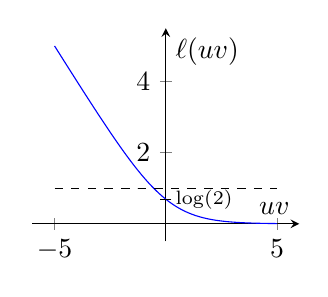
\begin{tikzpicture}
\begin{axis}[xlabel=$uv$,ylabel={$\ell(uv)$},axis lines=middle,enlargelimits,width=0.41\textwidth]
\addplot[samples=200,blue,smooth] {ln(1+exp(-x))};
\addplot[dashed] {1};
%\addplot[dashed] {ln(2)} node[right, font=\small] {$\log(2)$};
\addplot [black, mark=-, nodes near coords=$\log(2)$, font={\scriptsize}, every node near coord/.style={anchor=180}] coordinates {(0,{ln(2)})};
\end{axis}
\end{tikzpicture}%
} \quad
\subfloat[][\emph{Influence of the regularization term on the loss function, equation~\eqref{subeq:obj-fun}, $\lambda=\textcolor{blue}{1},\textcolor{red}{0.5},\textcolor{green}{0.1}$}\label{subfig:loss_regul}]%
{%
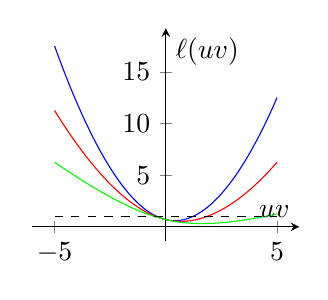
\begin{tikzpicture}
\begin{axis}[xlabel=$uv$,ylabel={$\ell(uv)$},axis lines=middle,enlargelimits,width=0.41\textwidth,legend style={nodes={scale=0.5, transform shape}}]
\addplot[samples=200,blue,smooth] {ln(1+exp(-x))+0.5*x^2};
\addplot[samples=200,red,smooth] {ln(1+exp(-x))+0.5*0.5*x^2};
\addplot[samples=200,green,smooth] {ln(1+exp(-x))+0.5*0.1*x^2};
\addplot[dashed] {1};
%\legend{$\lambda=1$, $\lambda=0.5$, $\lambda=0.1$}
\end{axis}
\end{tikzpicture}
} \quad
\subfloat[][\emph{Sigmoid function. Used for prediction with encoding: $\mathrm{if}\,v>0.5\Rightarrow\hat{u}=1$ and $\mathrm{if}\,v\leq0.5\Rightarrow\hat{u}=-1$.}\label{subfig:sigmoid}]%
{%
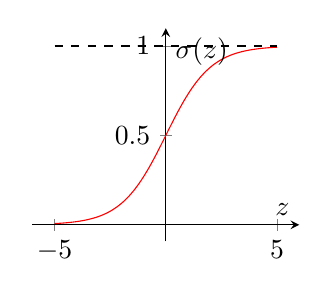
\begin{tikzpicture}
\begin{axis}[xlabel=$z$,ylabel={$\sigma(z)$},axis lines=middle,enlargelimits,width=0.41\textwidth]
\addplot[samples=200,red,smooth] {1/(1+exp(-x))};
\addplot[dashed] {1};
\end{axis}
\end{tikzpicture}%
}
\end{figure}

%\begin{itemize}
%\item $uv\gg0$: the example is labelled correctly
%\item $uv\ll0$: the class assigned to the example is the wrong one
%\end{itemize}

% !TeX spellcheck = en_GB
% ***************************************************** %
\section{Mini-batch gradient descent variants}
% ***************************************************** %

In this section we tackle the algorithmic part, the SGD-type chosen is the Mini-batch Gradient Descent where the mini-batch size $M$ is greater than 1 and much less than the dataset size, i.e. $1<\abs{B_t}=M\ll N$. For simplicity, we will call it SGD anyway.

The basic SGD performs steps of the form
\begin{equation}\label{eq:sgd_step}
w^{k+1}=w^k+\alpha_kd_k,\quad d_k=-\nabla f_{i_k}(w^k)
\end{equation}
where the direction $d_k$ is equal to the \emph{anti-gradient} evaluated on the considered sample (a random mini-batch extracted from the dataset), knowing that $\numberset{E}\bigl[\nabla f_{i_k}(w^k)\bigr]=\nabla\func(w)$, $d_k$ is a \emph{descent direction}. Also due to the global convergence, the algorithm can start from an arbitrary $w^0\in\R^{(p+1)}$.

Using this step-size form, without a line search method for choosing the optimal step-size $\alpha_k$, the objective function value doesn't decrease necessarily at each step, thus making the method \emph{non-monotonous}.

In order to use the SGD algorithm, it is necessary to make further assumptions on the objective function and the gradients (how far the gradient samples are from the \emph{true gradients})
\begin{itemize}
\item the function $f$ in problem~\eqref{eq:opt-prob} has a \emph{finite-sum structure}, that is the common machine learning setting;
\item being a loss function plus a quadratic regularization term, $f$ is bounded below by some value $f^\ast$, we can also take a look at figure~\ref{subfig:log-loss};
\item for some constant $G>0$ the magnitude of all gradients samples are bounded $\forall w\in\R^{(p+1)}$ by $\norma{\nabla f_i(w)}\leq G$;
\item other than twice continuously differentiable, we assume that $f$ has Lipschitz-continuous gradients with constant $L>0$, one can also say that $f$ is $L\text{-smooth}$.
\end{itemize}

Regarding the implementation of the algorithm, it is essential to define a stopping criterion. The first choice is always
\begin{equation}\label{eq:stopping1}
\norma{\nabla\func(w^k)}\leq\epsilon,\quad\epsilon>0
\end{equation}
unless there is a small tolerance $\epsilon$, the algorithm reaches a stationary point.

Other than this, we can add conditions of premature termination like
\begin{itemize}
\item exceeding a threshold for the epochs number $k^\ast$ or function and gradient evaluations;
\item internal failures when computing $w^{k+1}$, for example during the line search.
\end{itemize}


\subsubsection*{Mini-batch gradient}

Now we spend a few words about the computation of the mini-batch gradient evaluated on a point using the pseudo-code notation. Given a mini-batch $B_t$ at iteration $t$ with indices $i_t$ and the previous weights $y_t$, we want to compute
\begin{equation*}
%\begin{split}
%\nabla f_{i_t}(y_t) &= \frac{1}{M}\sum_{j\in B_t}\nabla f_j(y_t)\\
% &= \frac{1}{M}\sum_{j\in B_t}\bigl(x^{(j)}r_j+\lambda y\bigr) \\
% &= \frac{1}{M}\biggl(\sum_{j\in B_t}x^{(j)}r_j+M\lambda y\biggr) \\
% &= \frac{1}{M}\bigl(\underbrace{Xr}_{i_t\in B_t}+\lambda' y\bigr)
%\end{split}
\begin{split}
\nabla f_{i_t}(y_t) &= \frac{1}{M}\sum_{j\in B_t}\nabla f_j(y_t)=\frac{1}{M}\sum_{j\in B_t}\bigl(x^{(j)}r_j+\lambda y\bigr)= \frac{1}{M}\biggl(\sum_{j\in B_t}x^{(j)}r_j+M\lambda y\biggr) \\
 &= \frac{1}{M}\bigl(\underbrace{Xr}_{i_t\in B_t}+\lambda' y\bigr)
\end{split}
\end{equation*}
so we use the same expression as the full gradient except that the dataset matrix contains just the mini-batch samples (and so the $r$ vector), and the regularization coefficient is redefined as $\lambda'=M\lambda$ where $M$ is the size of the considered mini-batch.

% ---------------------------------------------------- %
\subsection{Stochastic gradient descent}
% ---------------------------------------------------- %

The SGD-type variants differs by the selection of the step-size. Particularly the basic version has two possible choices
\begin{itemize}
\item \emph{constant step-size} $\alpha_k=\alpha$;
\item \emph{decreasing step-size} $\alpha_k=\frac{\alpha_0}{k+1}$.
\end{itemize}
the second choice has such form in order to ensure the convergence of the algorithm; this two version are shown in algorithm~\vref{code:SGD-fix-decr}. The iteration~\eqref{eq:sgd_step} sees the index $k$ changed to $t$, the former is the index of the \emph{epochs} while the latter is the index of the mini-batches.

% ---------------------------------------------------- %
\subsubsection{Stochastic line search}
% ---------------------------------------------------- %

Now we move on to the approach by \texttt{bib1}. Other than $\mathcal{L}_0=\set{w\in\R^{(p+1)}\mid\func(w)\leq\func(w^0)}$ being a \emph{compact set}, since the function is coercive (see\dots), the proposed algorithm needs one more assumption, that is, the model is able to \emph{interpolate} the data, this property requires that the gradient w.r.t. each samples converges to zero at the optimal solution
\[
\text{if}\,\,\,w^\ast\mid\nabla\func(w^\ast)=0\Rightarrow\nabla f_i(w^\ast)=0\,\,\,\forall i=1,\dots,N
\]

The proposed approach applies the Armijo line search to the SGD algorithm, specializing the condition of sufficient reduction in the context of finite-sum problems. Referring to the notation in~\eqref{eq:sgd_step}, the \emph{Armijo condition} has the following form
\[
\func(w^{k+1})\leq\func(w^k)+\gamma\alpha_k\nabla\func(w^k)^Td_k\Rightarrow
f_{i_k}(w^{k+1})\leq f_{i_k}(w^k)+\gamma\alpha_k\nabla f_{i_k}(w^k)^Td_k
\]
so, when it comes to SGD we obtain
\begin{equation}\label{eq:armijo-sls}
f_{i_k}\bigl(w^k-\alpha_k\nabla f_{i_k}(w^k)\bigr)\leq f_{i_k}(w^k)-\gamma\alpha_k\nabla\norma{f_{i_k}(w^k)}^2
\end{equation}
as already said, $d_k$ is a \emph{descent direction}. The constant $\gamma$ is an hyper-parameter set to $1/2$ for convergence properties in the strongly-convex case.

As the standard Armijo method, the proposed line search uses a \emph{backtracking} technique that iteratively decreases the initial step-size $\alpha_0$ by a constant factor $\delta$ usually set to $1/2$ until the condition is satisfied.

The authors also gave heuristics in order to avoid unnecessary function evaluations by \emph{restarting} at each iteration the step-size, see algorithm~\vref{code:reset-step}.\footnote{\emph{Iterations} is defined as the total number of mini-batches extracted from the dataset, while one \emph{epoch} is when the entire dataset is passed forward.}

The SGD with Stochastic Line Search is shown in algorithm~\vref{code:SGD-Armijo}.

% ---------------------------------------------------- %
\subsection{Adding momentum term}
% ---------------------------------------------------- %

The iteration performed is still $w^{k+1}=w^k+\alpha_kd_k$ what differs from the basic versions is the direction
\[
d_k=-\bigl((1-\beta)\nabla f_{i_k}(w^k+\beta d_{k-1})\bigr)
\]
in a finite-sum problem the momentum term must be selected from a specific range $\beta\in(0,1)$, the algorithm is called SGDM, the resulting iteration
\begin{equation}\label{eq:sgdm-step}
w^{k+1}=w^k-\alpha_k\bigl((1-\beta)\nabla f_{i_k}(w^k+\beta d_{k-1})\bigr)
\end{equation}
which is applied in algorithm~\vref{code:SGDM}.

As the paper \texttt{bib2} says, when using the momentum term together with a line search, $\beta$ complicates the selection of a suitable step-size; using the algorithm~\ref{code:SGD-Armijo}, the approach is not robust to the choice of the momentum term.

Like the stochastic line search approach in section ..., the Armijo condition added to the SGDM algorithm has the form
\begin{equation}\label{eq:armijo-sgdm}
f_{i_k}(w^k+\alpha_kd_k)\leq f_{i_k}(w^k)-\gamma\alpha_k\nabla f_{i_k}(w^k)^T\bigl((1-\beta)\nabla f_{i_k}(w^k+\beta d_{k-1})\bigr)
\end{equation}
placing $d_{i_k}=-\nabla f_{i_k}(w^k)$ we obtain the equation~\eqref{eq:armijo-sls}.

The problem is that $\nabla f_{i_k}(w^k)^Td_{i_k}<0$ isn't always guaranteed, i.e. the direction is not descent, therefore the line search doesn't converge. There are thus two situations that can be resolved as follows
\begin{center}
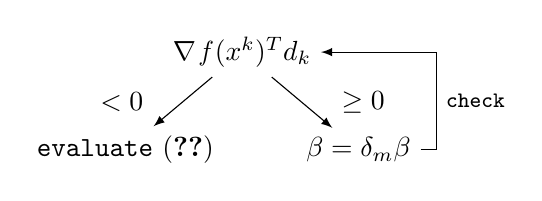
\begin{tikzpicture}
\node (A) at (0,0) {$\nabla\func(x^k)^Td_k$};
\node (B) at (-140:5.5em) {\texttt{evaluate}~\eqref{eq:armijo-sgdm}};
\node (C) at (-40:5.5em) {$\beta=\delta_m\beta$};
\draw[-latex] (A) -- node[left=2.5ex] {$<0$} (B);
\draw[-latex] (A) -- node[right=2.5ex] {$\geq0$} (C);
%\draw[-latex, bend right=55] (C.east) to (A.east);
\draw[-latex] (C.east) -- ++(0.2,0) -- node[right, font=\footnotesize] {\texttt{check}} ++(0,{5.5em*sin(40)}) -- (A.east);
\end{tikzpicture}
\end{center}
in algorithmic terms, while the direction is not descent, damp the momentum term by a factor $\delta_m$ usually set to $1/2$. Using this procedure, a descent direction $d_{i_k}$ is guaranteed, and is called \emph{momentum correction}, see algorithm~\vref{code:MSL-SGDM-C}.

This procedure can be expensive, so the paper suggests another approach called \emph{momentum restart}, when descent direction condition for $d_k$ isn't satisfied, the procedure sets $d_{k-1}=d_0=0$, see algorithm~\vref{code:MSL-SGDM-R}.
% !TeX spellcheck = en_GB
% ***************************************************** %
\section{Implementation}\label{sc:code}
% ***************************************************** %
%\cleardoublepage
% !TeX spellcheck = en_GB
% ***************************************************** %
\section{Experiments and results discussion}\label{sc:exp}
% ***************************************************** %

%\begin{table}
%\caption[]{Hyper-parameters}
%\label{tab:hyper-params}
%\[
%\begin{array}{l}
%\beta=0.9 \\
%\end{array}
%\]
%\end{table}

%\begin{figure}
%\centering
%\includegraphics[width=0.3\textwidth]{../py/test.pdf}
%\end{figure}

% df.to_latex

To test the efficiency the algorithms, a benchmark of six datasets retrieved from \href{https://www.csie.ntu.edu.tw/~cjlin/libsvmtools/datasets/}{LIBSVM} is used, see table~\vref{tab:datasets} for details.

First the six algorithms are tested on a fixed number of epochs, \textcite{fan_msl_2023} set the value to \num{200}, so we do the same. We keep track of the loss function value for every epoch and the running time that every epoch took; our aim is to show how the value decreases on every epoch and the running time that takes, see figures on pages~\pageref{fig:diab-breast}, \pageref{fig:phish-austr} and \pageref{fig:mush-german}.\par\smallskip

Once we have the algorithms performance at different step-size values, a fine-tuning of the hyper-parameter is done in order to obtain the best solver for every dataset based on the accuracy score and loss function values. For a better comparison, the L-BFGS, Conjugate Gradient and Newton-CG, and the full-batch gradient descent algorithms are also tested.

The only hyper-parameter that varies is the step-size $\alpha$, the momentum term is set to \num{0.9}, the mini-batch size is a power of 2 and is set according to perform at least \num{100} \emph{iterations} depending on the considered dataset and the $\epsilon$ tolerance from~\eqref{eq:stopping} is set to \num{e-3}.

% grid search
% i valori "ottimi" della grid search per i parametri che non sono il learning rate sono stati usati per mostrare poi l'andamento al variare del learning rate

\begin{table}
\centering
\caption{Benchmark datasets}
\label{tab:datasets}
\begin{tabular}{lSSSc}
\toprule
Name & {Train} & {Test} & {Features} & {Distribution} \\
\midrule
w1a & 2477 & 47272 & 300 & -1:$0.97$\,\,\,1:$0.03$ \\
w3a & 4912 & 44837 & 300 & -1:$0.97$\,\,\,1:$0.03$ \\
Phishing & 8844 & 2211 & 68 & -1:$0.45$\,\,\,1:$0.55$ \\
a2a & 2265 & 30296 & 119 & -1:$0.75$\,\,\,1:$0.25$ \\
Mushrooms & 6499 & 1625 & 112 & -1:$0.48$\,\,\,1:$0.52$ \\
German & 800 & 200 & 24 & -1:$0.70$\,\,\,1:$0.30$ \\
\bottomrule
\end{tabular}
\end{table}

%\cleardoublepage
\begin{table}
\sisetup{round-mode=places}
\centering
\caption{w1a dataset}
\label{tab:w1a-table}
\begin{tabular}{lS[round-precision=3]S[drop-zero-decimal]S[round-precision=4]S[round-precision=6]S[exponent-mode=scientific]S[round-precision=6]}
\toprule
Solver & {$\alpha_0$} & {Epochs} & {Run-time} & {$\func(w)$} & {$\nabla f(w)$} & {Test score} \\
\midrule
Newton-CG & NaN & 6 & NaN & 0.464614 & 0.000046 & 0.970236 \\
CG & NaN & 7 & NaN & 0.464614 & 0.000009 & 0.970236 \\
L-BFGS-B & NaN & 7 & NaN & 0.464614 & 0.000023 & 0.970236 \\
BatchGD-Fixed & 1.000000 & 12 & 0.010029 & 0.464614 & 0.000564 & 0.970236 \\
SGD-Decreasing & 0.500000 & 27 & 0.214942 & 0.464614 & 0.000792 & 0.970236 \\
SGD-Fixed & 0.010000 & 27 & 0.186510 & 0.464615 & 0.000852 & 0.970236 \\
SGDM & 0.010000 & 386 & 5.914988 & 0.464615 & 0.000978 & 0.970236 \\
MSL-SGDM-R & 0.005000 & 600 & 6.497748 & 0.464693 & 0.009144 & 0.970236 \\
MSL-SGDM-C & 0.005000 & 600 & 6.388432 & 0.464693 & 0.009149 & 0.970236 \\
SGD-Armijo & 0.100000 & 600 & 7.664835 & 0.536467 & 0.363829 & 0.971400 \\
\bottomrule
\end{tabular}
\end{table}

\begin{table}
\sisetup{round-mode=places}
\centering
\caption{w3a dataset}
\label{tab:w3a-tab}
\begin{tabular}{lS[round-precision=3]S[drop-zero-decimal]S[round-precision=4]S[round-precision=6]S[exponent-mode=scientific]S[round-precision=6]}
\toprule
Solver & {$\alpha_0$} & {Epochs} & {Run-time} & {$\func(w)$} & {$\nabla f(w)$} & {Test score} \\
\midrule
Newton-CG & NaN & 6 & NaN & 0.462742 & 0.000011 & 0.970203 \\
CG & NaN & 7 & NaN & 0.462742 & 0.000022 & 0.970203 \\
L-BFGS-B & NaN & 7 & NaN & 0.462742 & 0.000033 & 0.970203 \\
BatchGD-Fixed & 1.000000 & 12 & 0.016491 & 0.462742 & 0.000564 & 0.970203 \\
SGD-Decreasing & 0.500000 & 19 & 0.081762 & 0.462743 & 0.000876 & 0.970203 \\
SGD-Fixed & 0.010000 & 23 & 0.162157 & 0.462743 & 0.000949 & 0.970203 \\
SGDM & 0.100000 & 45 & 0.351333 & 0.462743 & 0.000895 & 0.970203 \\
MSL-SGDM-C & 0.005000 & 600 & 4.021617 & 0.462787 & 0.006924 & 0.970203 \\
MSL-SGDM-R & 0.005000 & 600 & 4.124630 & 0.462787 & 0.006924 & 0.970203 \\
SGD-Armijo & 0.010000 & 600 & 6.851229 & 0.500431 & 0.268456 & 0.971006 \\
\bottomrule
\end{tabular}
\end{table}

\begin{table}
\sisetup{round-mode=places}
\caption{Phishing dataset}
\label{tab:phish-tab}
\centering
\begin{tabular}{lS[round-precision=3]S[drop-zero-decimal]S[round-precision=4]S[round-precision=6]S[exponent-mode=scientific]S[round-precision=6]}
\toprule
Solver & {$\alpha_0$} & {Epochs} & {Run-time} & {$\func(w)$} & {$\nabla f(w)$} & {Test score} \\
\midrule
Newton-CG & NaN & 5 & NaN & 0.685065 & 0.000000 & 0.567616 \\
L-BFGS-B & NaN & 5 & NaN & 0.685065 & 0.000008 & 0.567616 \\
CG & NaN & 6 & NaN & 0.685065 & 0.000023 & 0.567616 \\
SGD-Decreasing & 0.100000 & 6 & 0.040321 & 0.685065 & 0.000508 & 0.567616 \\
SGDM & 0.100000 & 22 & 0.271079 & 0.685065 & 0.000575 & 0.567616 \\
BatchGD-Fixed & 1.000000 & 11 & 0.055085 & 0.685065 & 0.000534 & 0.567616 \\
SGD-Fixed & 0.010000 & 13 & 0.173696 & 0.685065 & 0.000927 & 0.567616 \\
MSL-SGDM-R & 0.100000 & 600 & 17.498211 & 0.685660 & 0.032621 & 0.568521 \\
MSL-SGDM-C & 1.000000 & 600 & 9.598539 & 0.685705 & 0.032668 & 0.568973 \\
SGD-Armijo & 0.005000 & 600 & 7.578606 & 0.687736 & 0.066541 & 0.865219 \\
\bottomrule
\end{tabular}
\end{table}

\begin{table}
\sisetup{round-mode=places}
\caption{a2a dataset}
\label{tab:a2a-tab}
\centering
\begin{tabular}{lS[round-precision=3]S[drop-zero-decimal]S[round-precision=4]S[round-precision=6]S[exponent-mode=scientific]S[round-precision=6]}
\toprule
Solver & {$\alpha_0$} & {Epochs} & {Run-time} & {$\func(w)$} & {$\nabla f(w)$} & {Test score} \\
\midrule
Newton-CG & NaN & 5 & NaN & 0.564027 & 0.000004 & 0.760265 \\
CG & NaN & 12 & NaN & 0.564027 & 0.000015 & 0.760265 \\
L-BFGS-B & NaN & 8 & NaN & 0.564027 & 0.000012 & 0.760265 \\
SGD-Decreasing & 0.800000 & 59 & 0.183221 & 0.564028 & 0.000726 & 0.760265 \\
SGDM & 0.100000 & 600 & 1.873068 & 0.564030 & 0.002628 & 0.760298 \\
MSL-SGDM-R & 0.010000 & 600 & 7.889470 & 0.577575 & 0.228297 & 0.790236 \\
MSL-SGDM-C & 0.010000 & 600 & 7.482898 & 0.579879 & 0.229332 & 0.789345 \\
BatchGD-Fixed & 1.000000 & 600 & 0.260017 & 0.594416 & 0.363976 & 0.822386 \\
SGD-Fixed & 1.000000 & 600 & 4.331557 & 0.602741 & 0.356183 & 0.807136 \\
SGD-Armijo & 1.000000 & 600 & 6.068792 & 0.617908 & 0.433035 & 0.798917 \\
\bottomrule
\end{tabular}
\end{table}

\begin{table}
\sisetup{round-mode=places}
\caption{Mushrooms dataset}
\label{tab:mush-tab}
\centering
\begin{tabular}{lS[round-precision=3]S[drop-zero-decimal]S[round-precision=4]S[round-precision=6]S[exponent-mode=scientific]S[round-precision=6]}
\toprule
Solver & {$\alpha_0$} & {Epochs} & {Run-time} & {$\func(w)$} & {$\nabla f(w)$} & {Test score} \\
\midrule
Newton-CG & NaN & 7 & NaN & 0.517726 & 0.000003 & 0.892923 \\
CG & NaN & 11 & NaN & 0.517726 & 0.000024 & 0.892923 \\
L-BFGS-B & NaN & 10 & NaN & 0.517726 & 0.000017 & 0.892923 \\
SGD-Decreasing & 0.100000 & 26 & 0.533000 & 0.517727 & 0.000779 & 0.893538 \\
BatchGD-Fixed & 0.500000 & 26 & 0.059922 & 0.517727 & 0.000757 & 0.892923 \\
SGD-Fixed & 0.500000 & 600 & 2.993838 & 0.525499 & 0.199874 & 0.926154 \\
MSL-SGDM-R & 0.100000 & 600 & 7.885503 & 0.527069 & 0.232121 & 0.940308 \\
MSL-SGDM-C & 0.100000 & 600 & 13.411705 & 0.527262 & 0.223900 & 0.939692 \\
SGD-Armijo & 0.100000 & 600 & 11.367419 & 0.535765 & 0.233549 & 0.953231 \\
SGDM & 1.000000 & 600 & 4.369383 & 0.557069 & 0.479065 & 0.924308 \\
\bottomrule
\end{tabular}
\end{table}

\begin{table}
\sisetup{round-mode=places}
\caption{German dataset}
\label{tab:german-tab}
\centering
\begin{tabular}{lS[round-precision=3]S[drop-zero-decimal]S[round-precision=4]S[round-precision=6]S[exponent-mode=scientific]S[round-precision=6]}
\toprule
Solver & {$\alpha_0$} & {Epochs} & {Run-time} & {$\func(w)$} & {$\nabla f(w)$} & {Test score} \\
\midrule
Newton-CG & NaN & 5 & NaN & 0.597303 & 0.000010 & 0.710000 \\
CG & NaN & 12 & NaN & 0.597303 & 0.000004 & 0.710000 \\
L-BFGS-B & NaN & 7 & NaN & 0.597303 & 0.000014 & 0.710000 \\
SGD-Fixed & 0.010000 & 58 & 0.129290 & 0.597303 & 0.000775 & 0.710000 \\
BatchGD-Fixed & 0.500000 & 20 & 0.011878 & 0.597303 & 0.000882 & 0.710000 \\
MSL-SGDM-R & 0.005000 & 600 & 2.221751 & 0.597456 & 0.023193 & 0.710000 \\
MSL-SGDM-C & 0.005000 & 600 & 2.861868 & 0.607466 & 0.140436 & 0.735000 \\
SGD-Decreasing & 0.010000 & 600 & 2.867500 & 0.607993 & 0.113583 & 0.720000 \\
SGD-Armijo & 0.100000 & 600 & 2.484220 & 0.614589 & 0.229813 & 0.740000 \\
SGDM & 1.000000 & 600 & 2.522513 & 0.616375 & 0.313714 & 0.745000 \\
\bottomrule
\end{tabular}
\end{table}

\begin{figure}
\centering
% w1a
\subfloat[][\emph{w1a dataset}\label{subfig:w1a-diagnostic}]%
{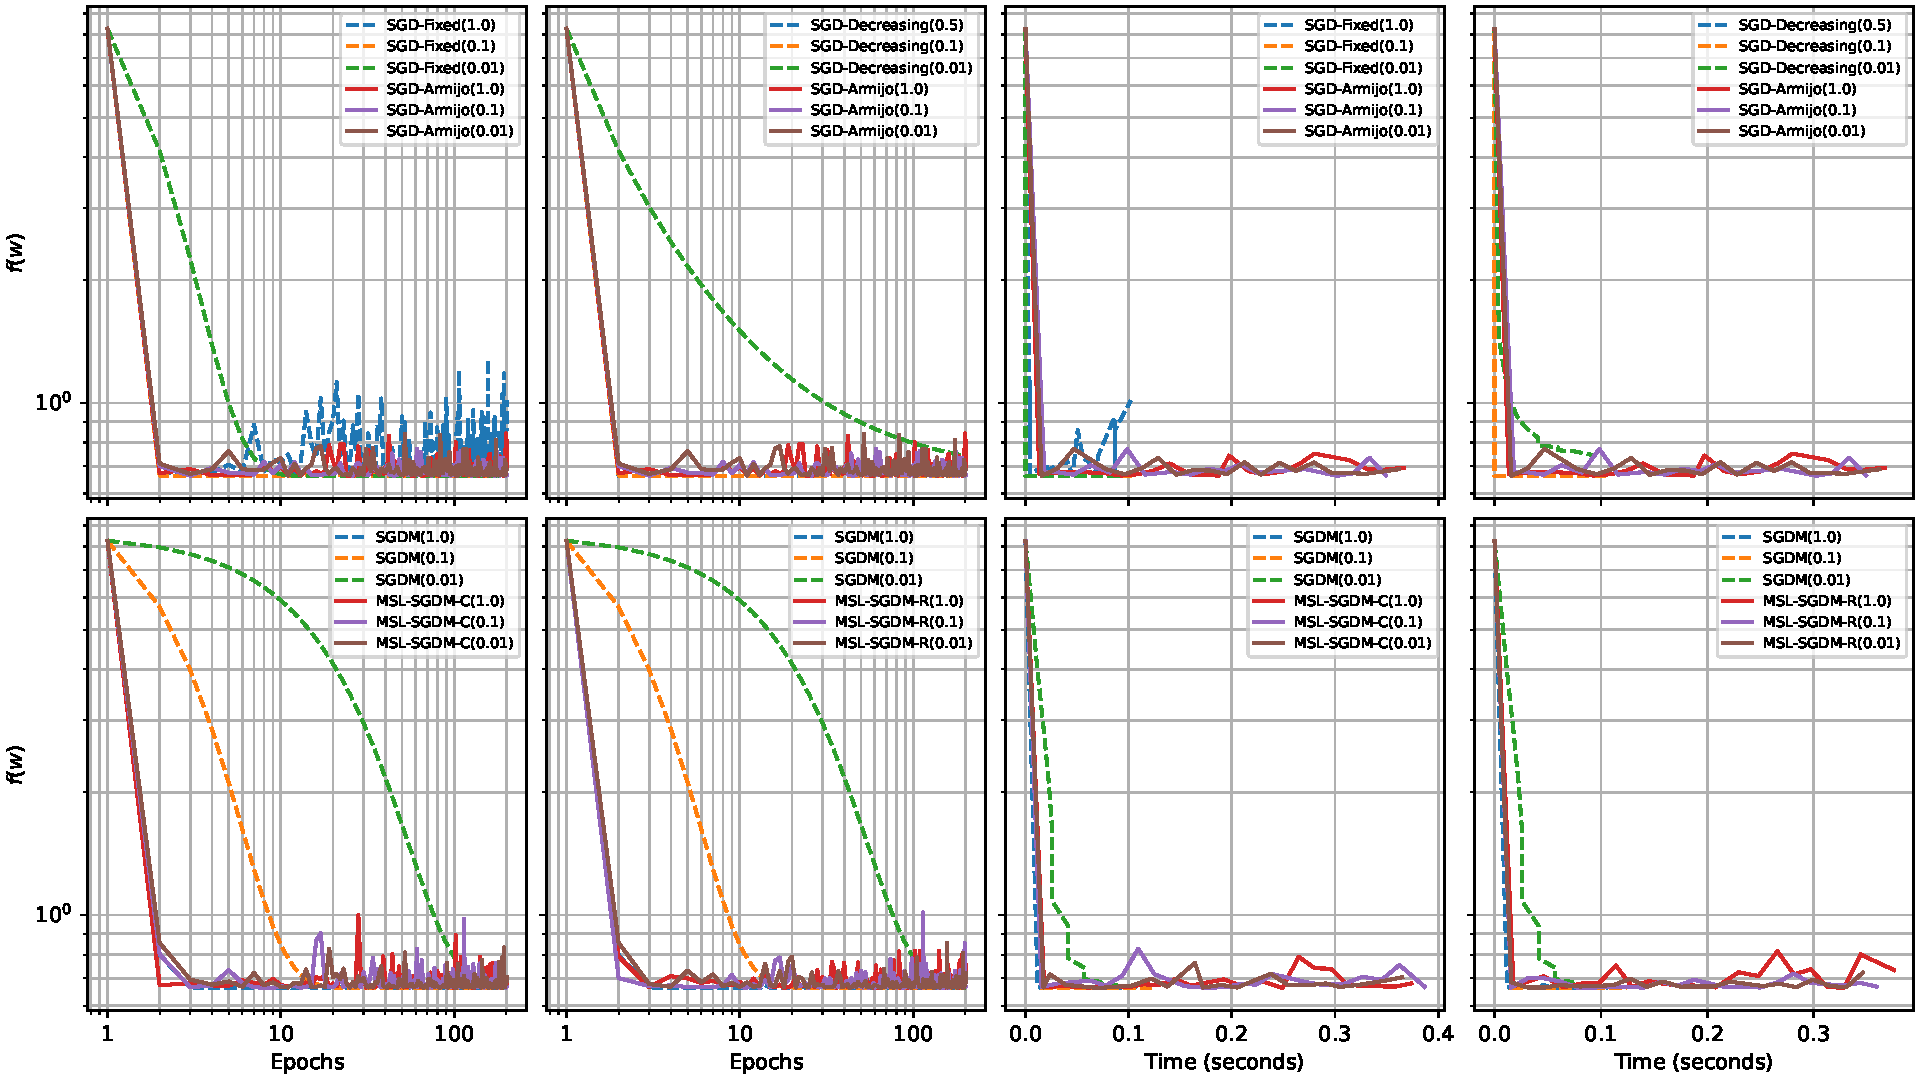
\includegraphics[width=\textwidth]{diab-diagnostic}} \\
% w3a
\subfloat[][\emph{w3a dataset}\label{subfig:w3a-diagnostic}]%
{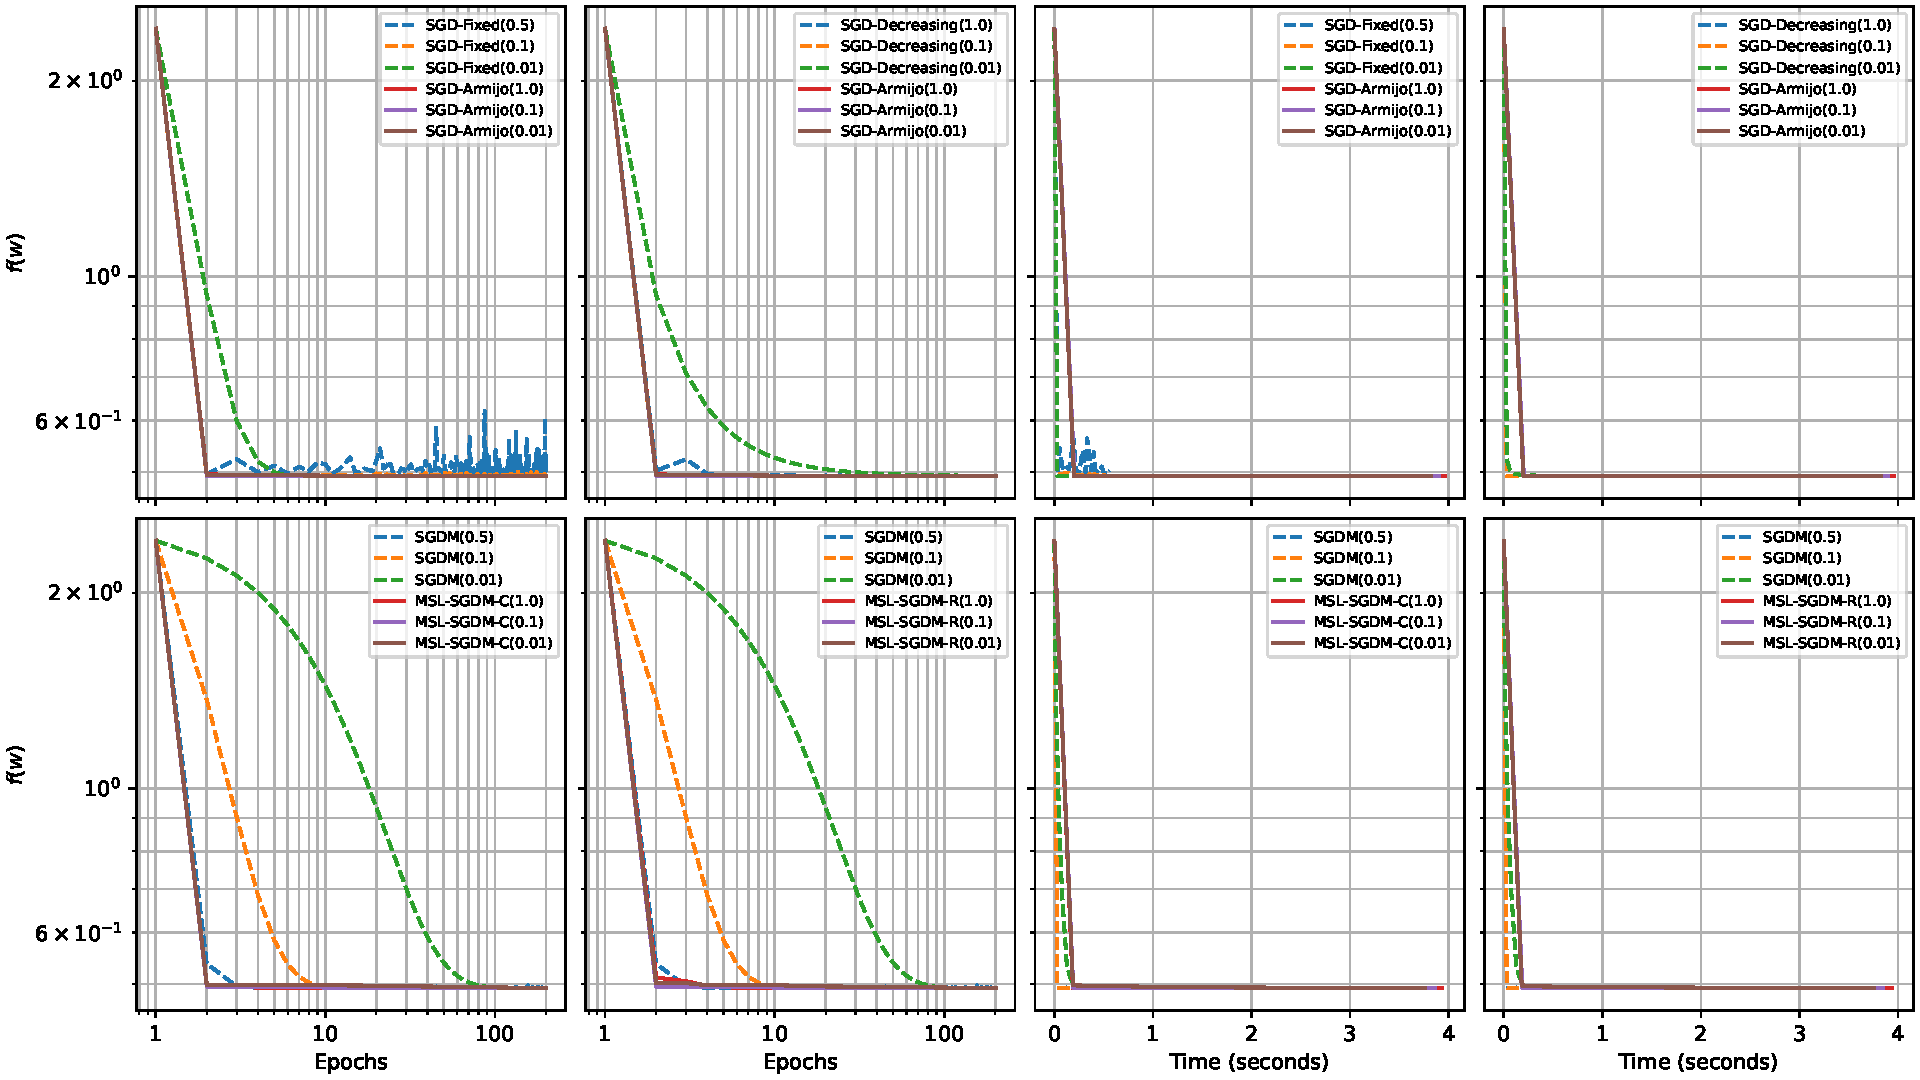
\includegraphics[width=\textwidth]{breast-diagnostic}} \\
\caption[]{w1a and w3ar}
\label{fig:diab-breast}
\end{figure}

\begin{figure}
\centering
% Phishing
\subfloat[][\emph{Phishing dataset}\label{subfig:phish-diagnostic}]%
{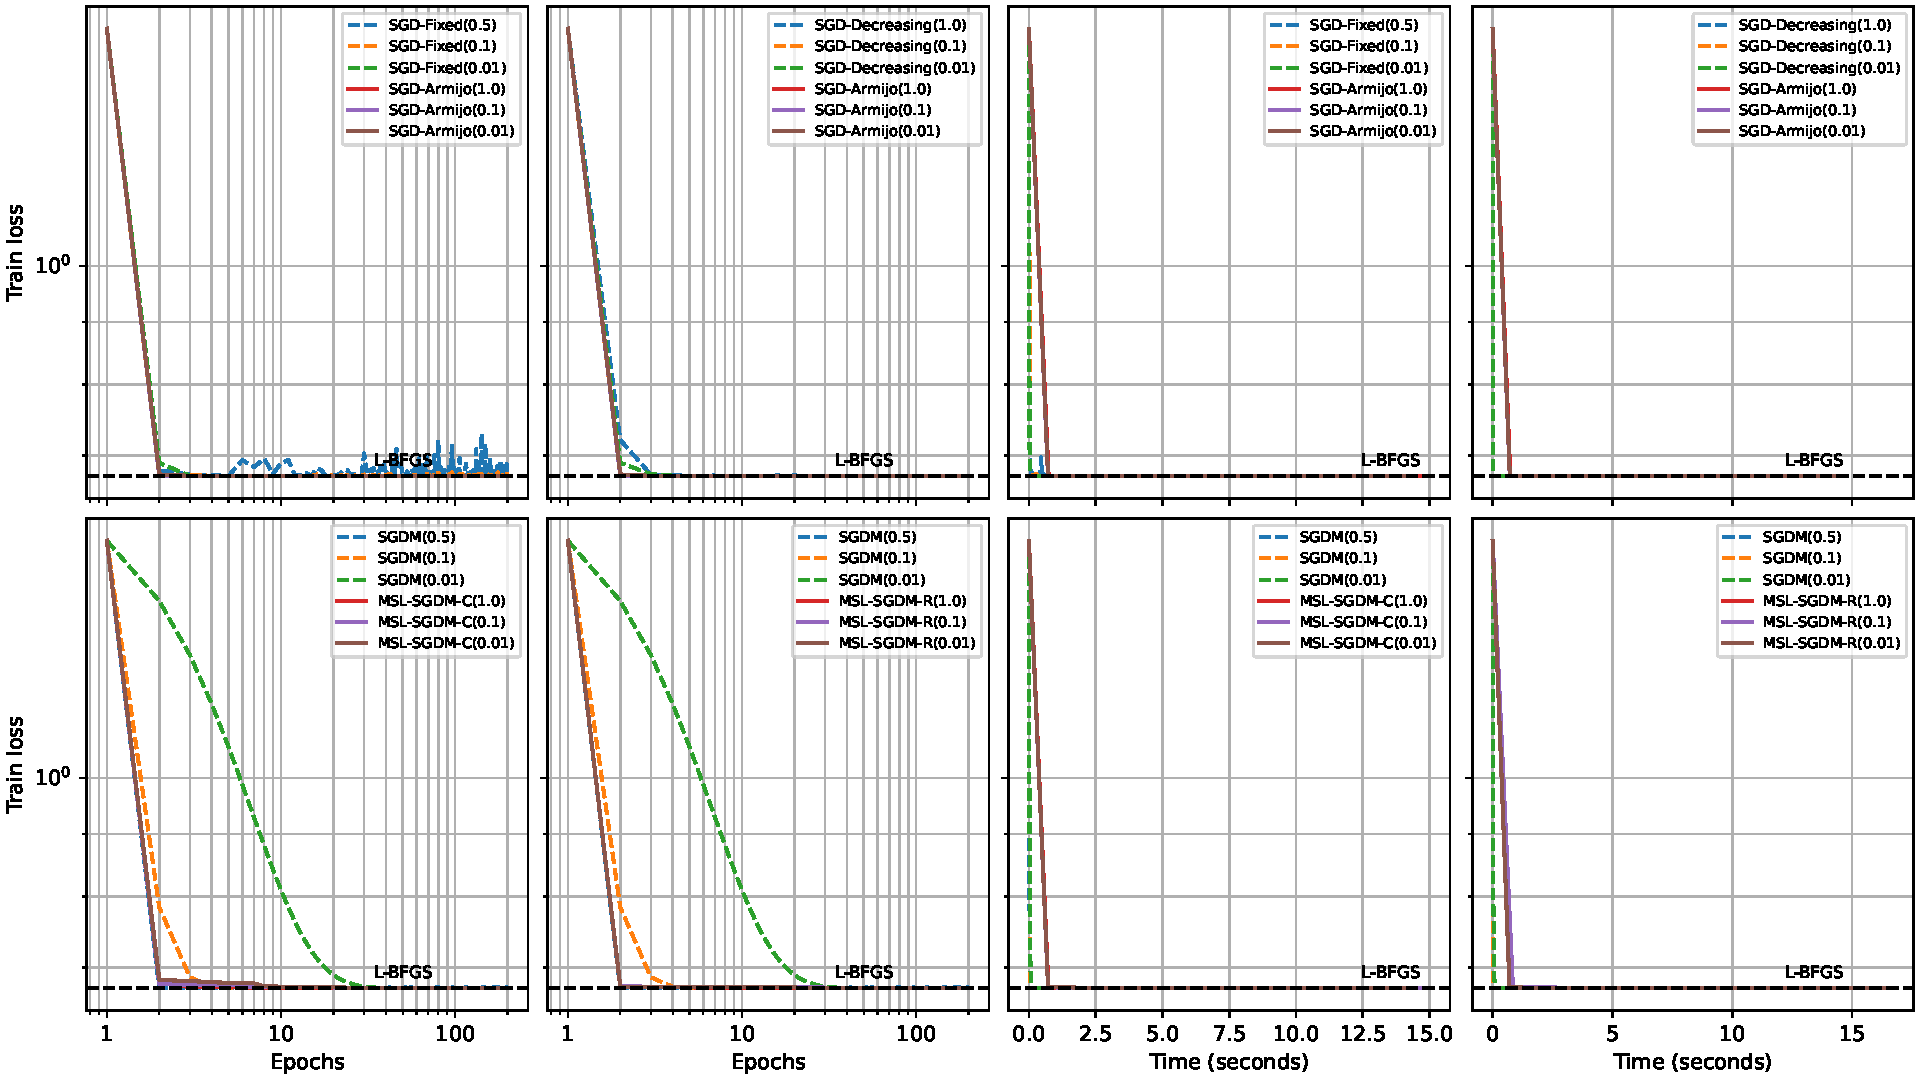
\includegraphics[width=\textwidth]{svm-diagnostic}} \\
% a2a
\subfloat[][\emph{a2a dataset}\label{subfig:a2a-diagnostic}]%
{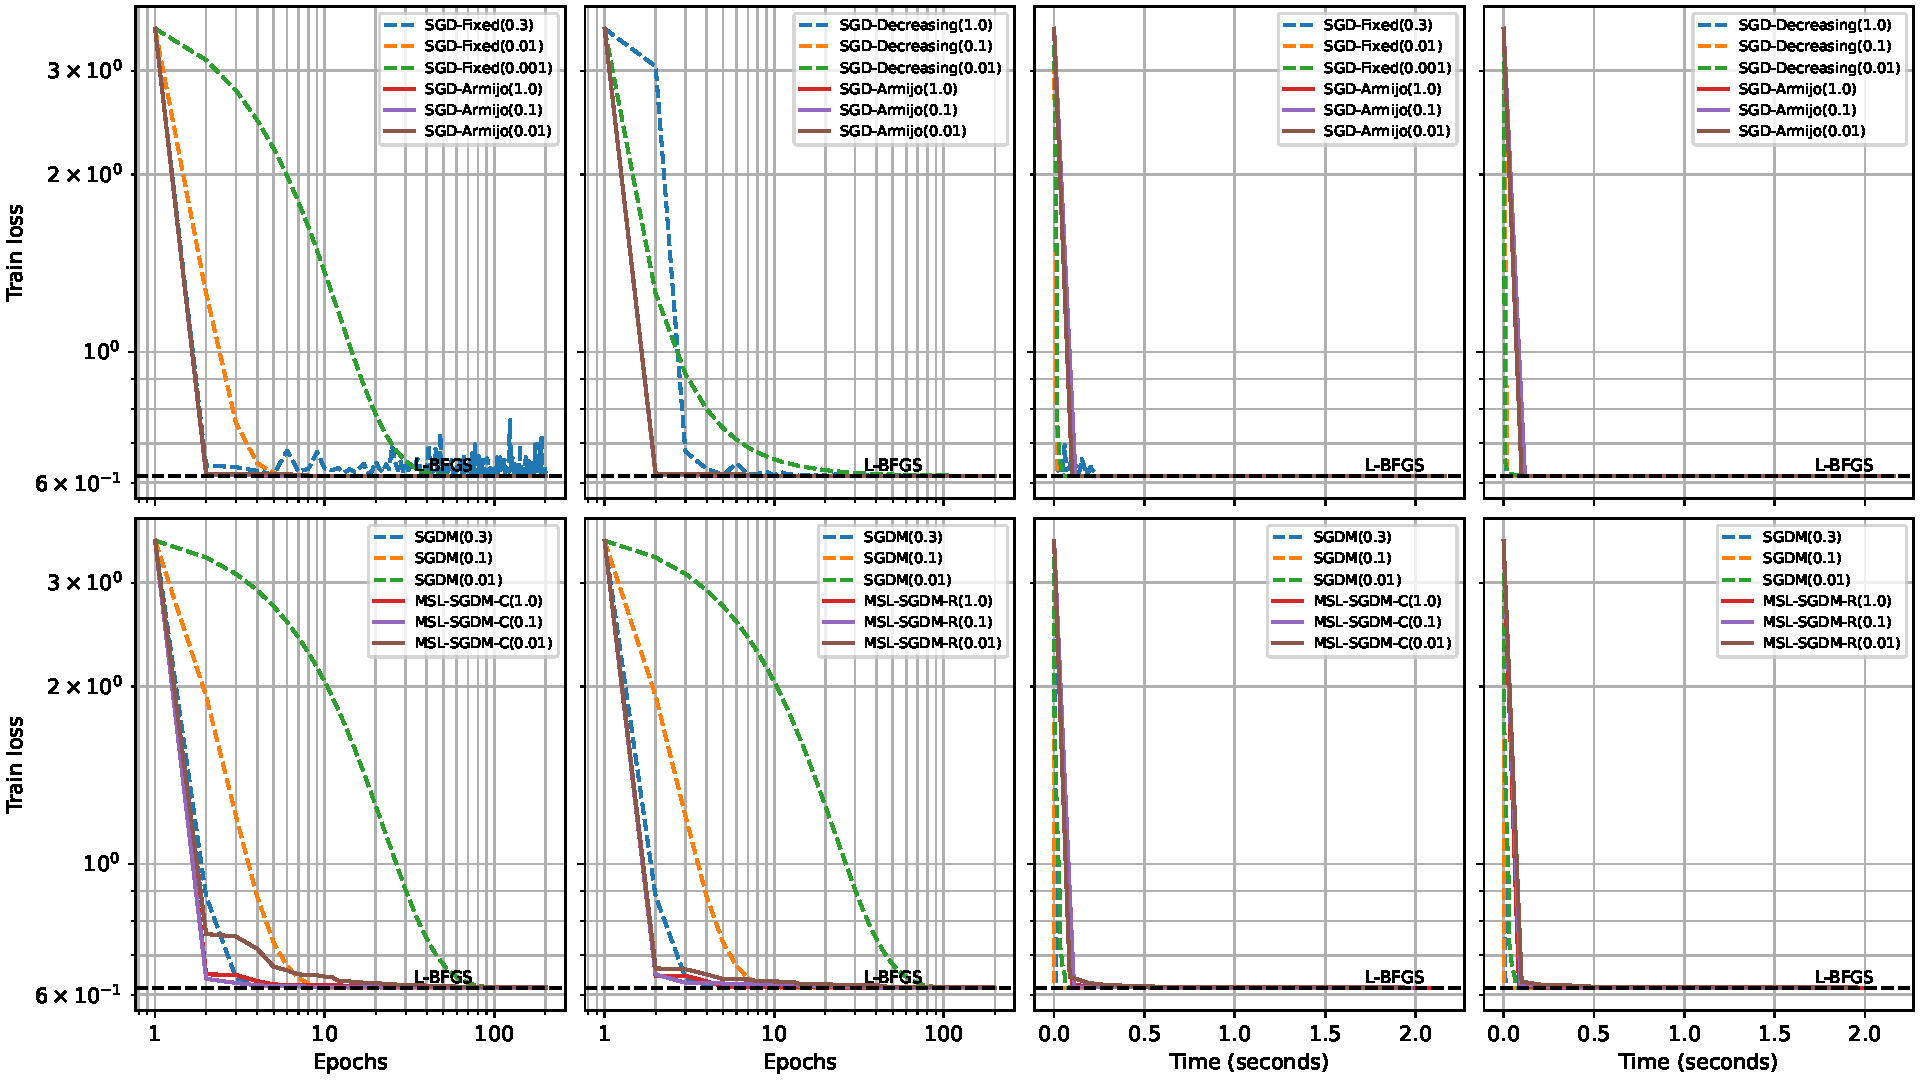
\includegraphics[width=\textwidth]{austr-diagnostic}}
\caption[]{Phishing and a2a datasets}
\label{fig:phish-austr}
\end{figure}

\begin{figure}
\centering
% mushrooms
\subfloat[][\emph{Mushrooms dataset}\label{subfig:mush-diagnostic}]%
{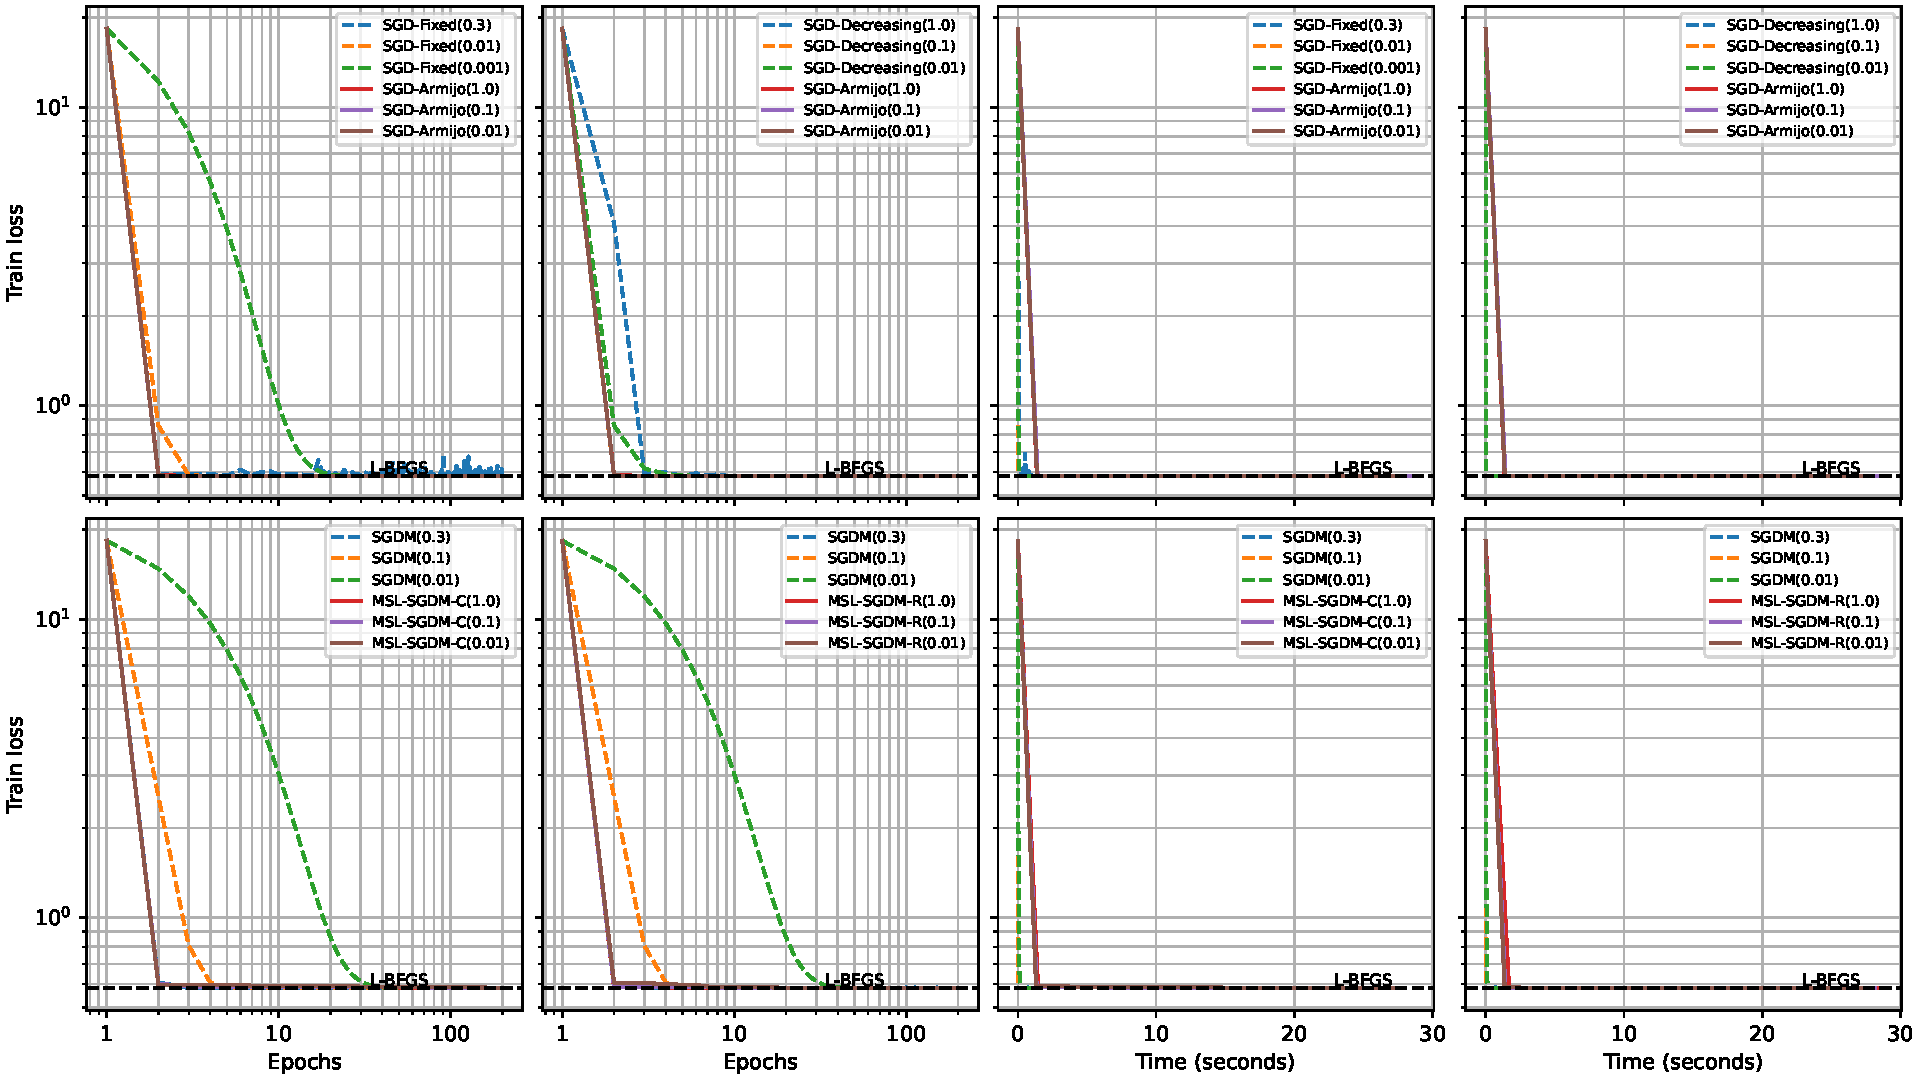
\includegraphics[width=\textwidth]{mush-diagnostic}} \\
% german
\subfloat[][\emph{German dataset}\label{subfig:german-diagnostic}]%
{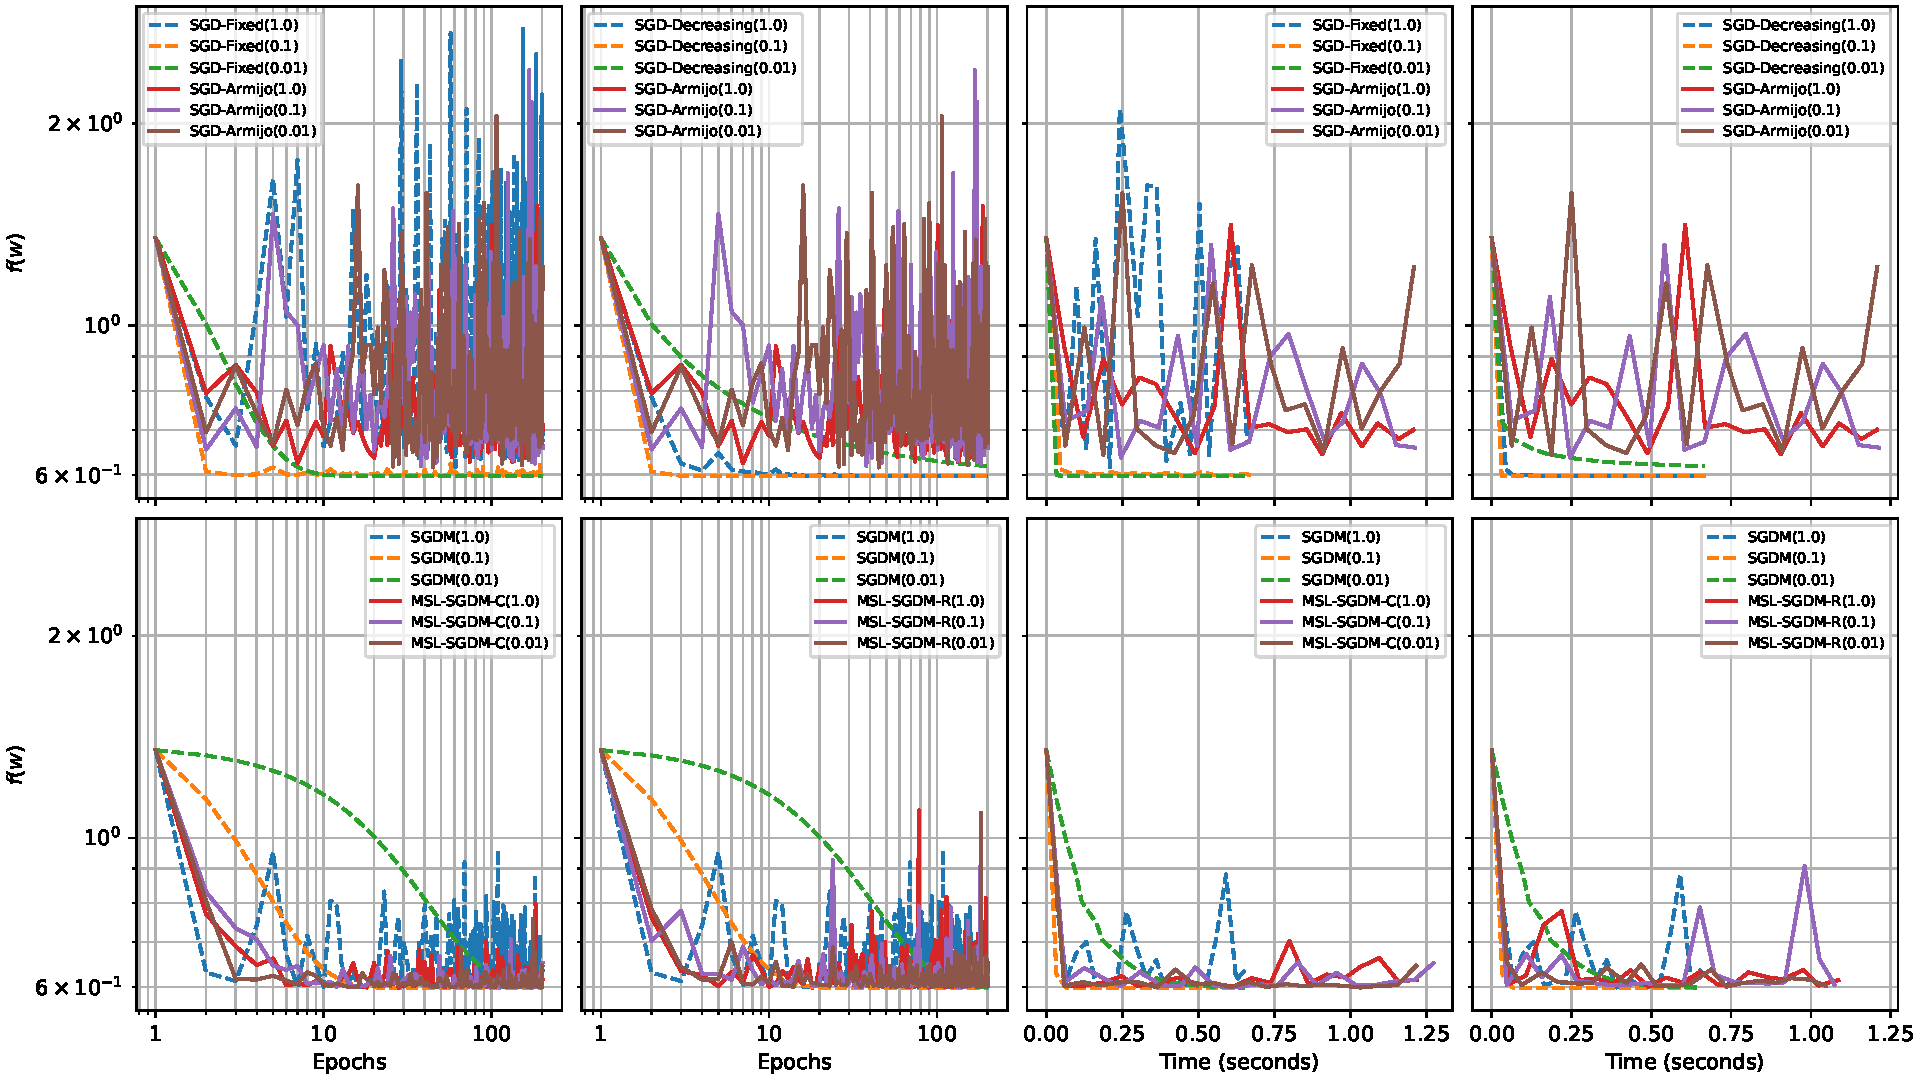
\includegraphics[width=\textwidth]{german-diagnostic}}
\caption[]{Mushrooms and German datasets}
\label{fig:mush-german}
\end{figure}

%\cleardoublepage
% ***************************************************** %
%\section{Mathematical background}
% ***************************************************** %

%\begin{defs}[Convex function]\label{def:conv_fun}
%	Let $S\subseteq\R^n$ be a convex set, a function $f\colon S\to\R$ is said to be convex if the hessian matrix is semi-positive-defined. If the hessian matrix is positive-defined, then the function is strictly convex.
%\end{defs}
%
%\begin{thm}[Weirstrass theorem]\label{thm:weirs}
%	Let $f\colon\R^n\to\R$ be a continuous function and $S\subseteq\R^n$ a compact set. Then function $f$ admits global minimum in $S$.
%\end{thm}
%
%\begin{cor}[Sufficient condition]\label{cor:weirs1}
%	If function $f\colon\R^n\to\R$ is a continuous and coercive function, then $f$ admits global minimum in $\R^n$.
%\end{cor}
%
%\begin{prop}[Coercivity of a quadratic function]
%	A quadratic function $\func(x)=\frac{1}{2}x^TQx-c^Tx$ is said to be coercive if and only if the symmetric matrix $Q\in\R^{n\times n}$ is positive-defined.
%\end{prop}
%
%\begin{prop}[Unique global minimum]\label{prop:min_unique}
%	Let $S\subseteq\R^n$ be a convex set, let $f\colon S\to\R$ be a strictly convex function. Then the global minimum, if exists, is unique.
%\end{prop}
%
%\begin{prop}[First order optimality condition]
%	$\bar{x}$ is a local minimum for $f\colon\R^n\to\R$ of class $f\in C^1(\R^n)$ if and only if $\nabla\func(\bar{x})=0$.
%\end{prop}
%
%\begin{prop}[Second order optimality condition]\label{prop:opt_second}
%	$\bar{x}\in\R^n$ is a local minimum for $f\colon\R^n\to\R$ of class $f\in C^2(\R^n)$ if and only if
%	\[\nabla\func(\bar{x})=0\quad\wedge\quad \nabla^2\func(\bar{x})\,\,\,\text{positive semi-definite}\]
%\end{prop}

% add definition of coercive function and proposition about compact sets?
% add gradient descent?
\cleardoublepage
%% !TeX spellcheck = en_GB
% ***************************************************** %
\section{Implementation}\label{sc:code}
% ***************************************************** %

% ************************************************************************************* %
% BACKMATTER %
% ************************************************************************************* %
\phantomsection
\inToc{\refname}
\printbibliography
\end{document}
